\begin{figure*}[t]
\centering
\begin{minipage}[t]{0.315\textwidth}\centering
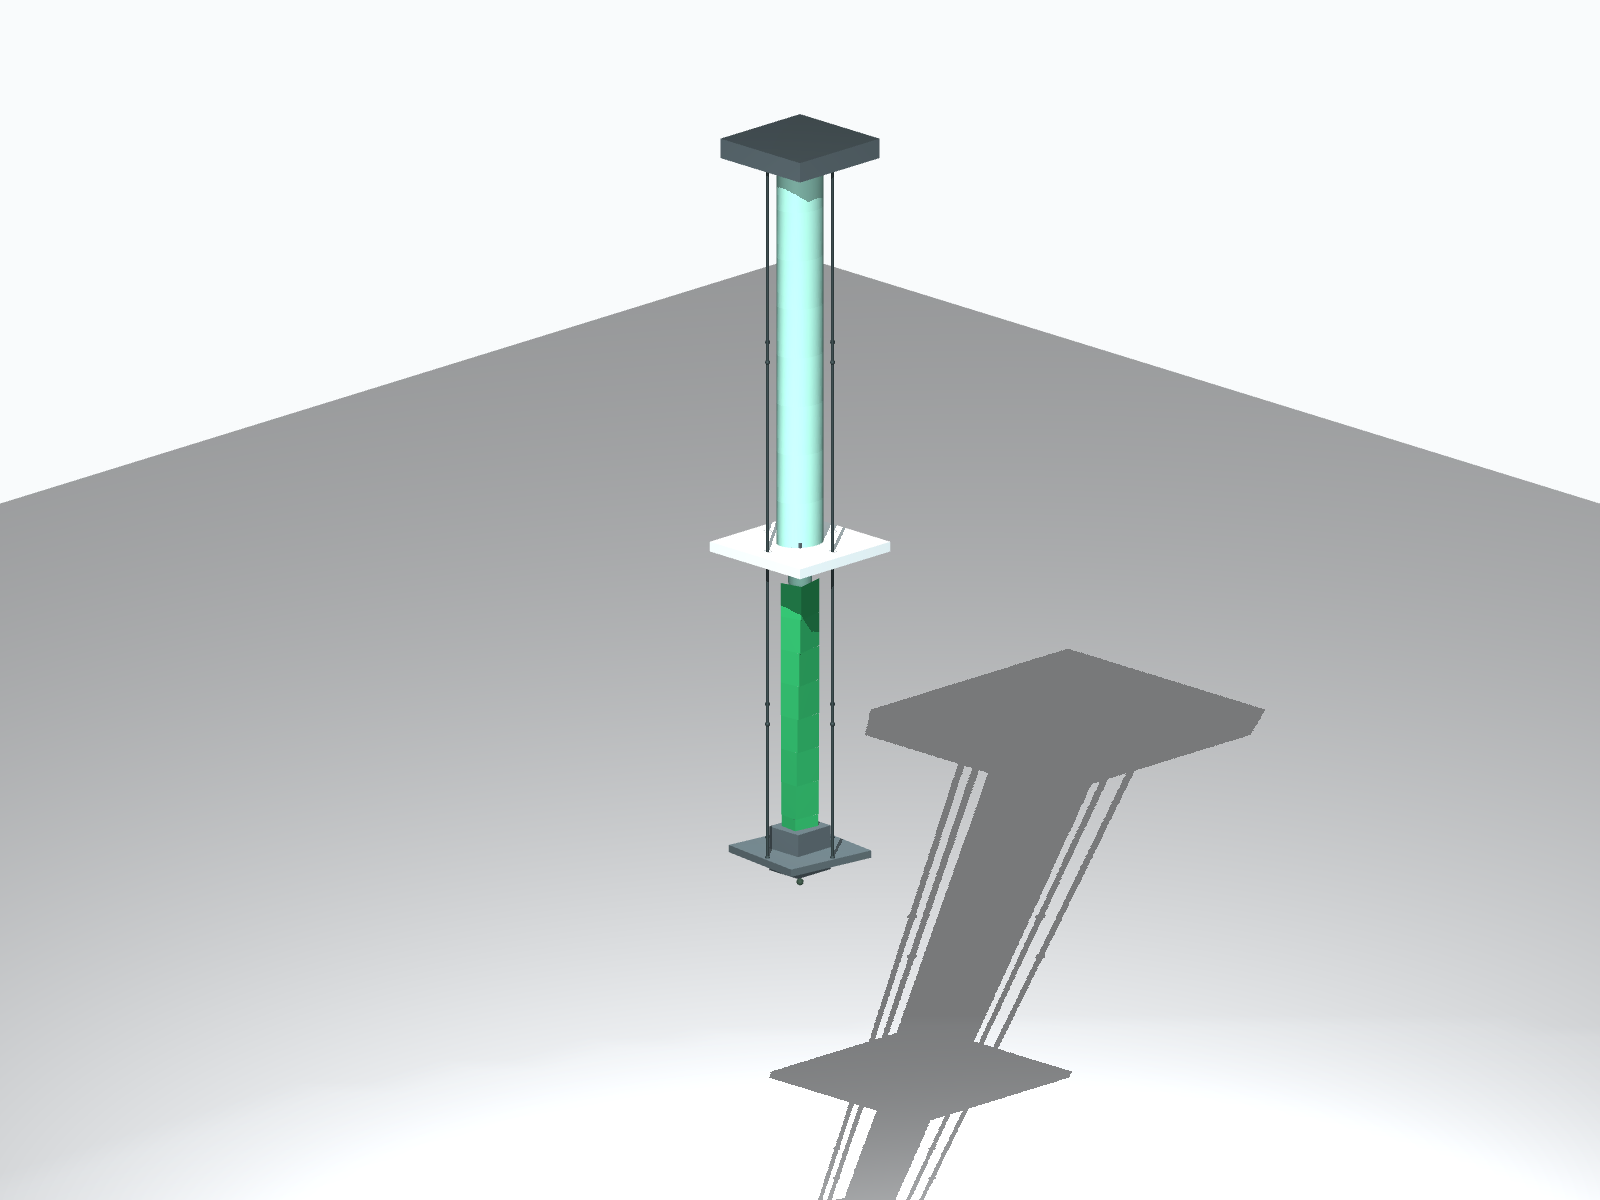
\includegraphics[width=\linewidth]{figures/native/phs2d_initial.png}
\par\footnotesize (a) Initial diagnostic
\par\scriptsize \textit{Evidence:} Local constraint insufficient
\end{minipage}\hfill
\begin{minipage}[t]{0.315\textwidth}\centering
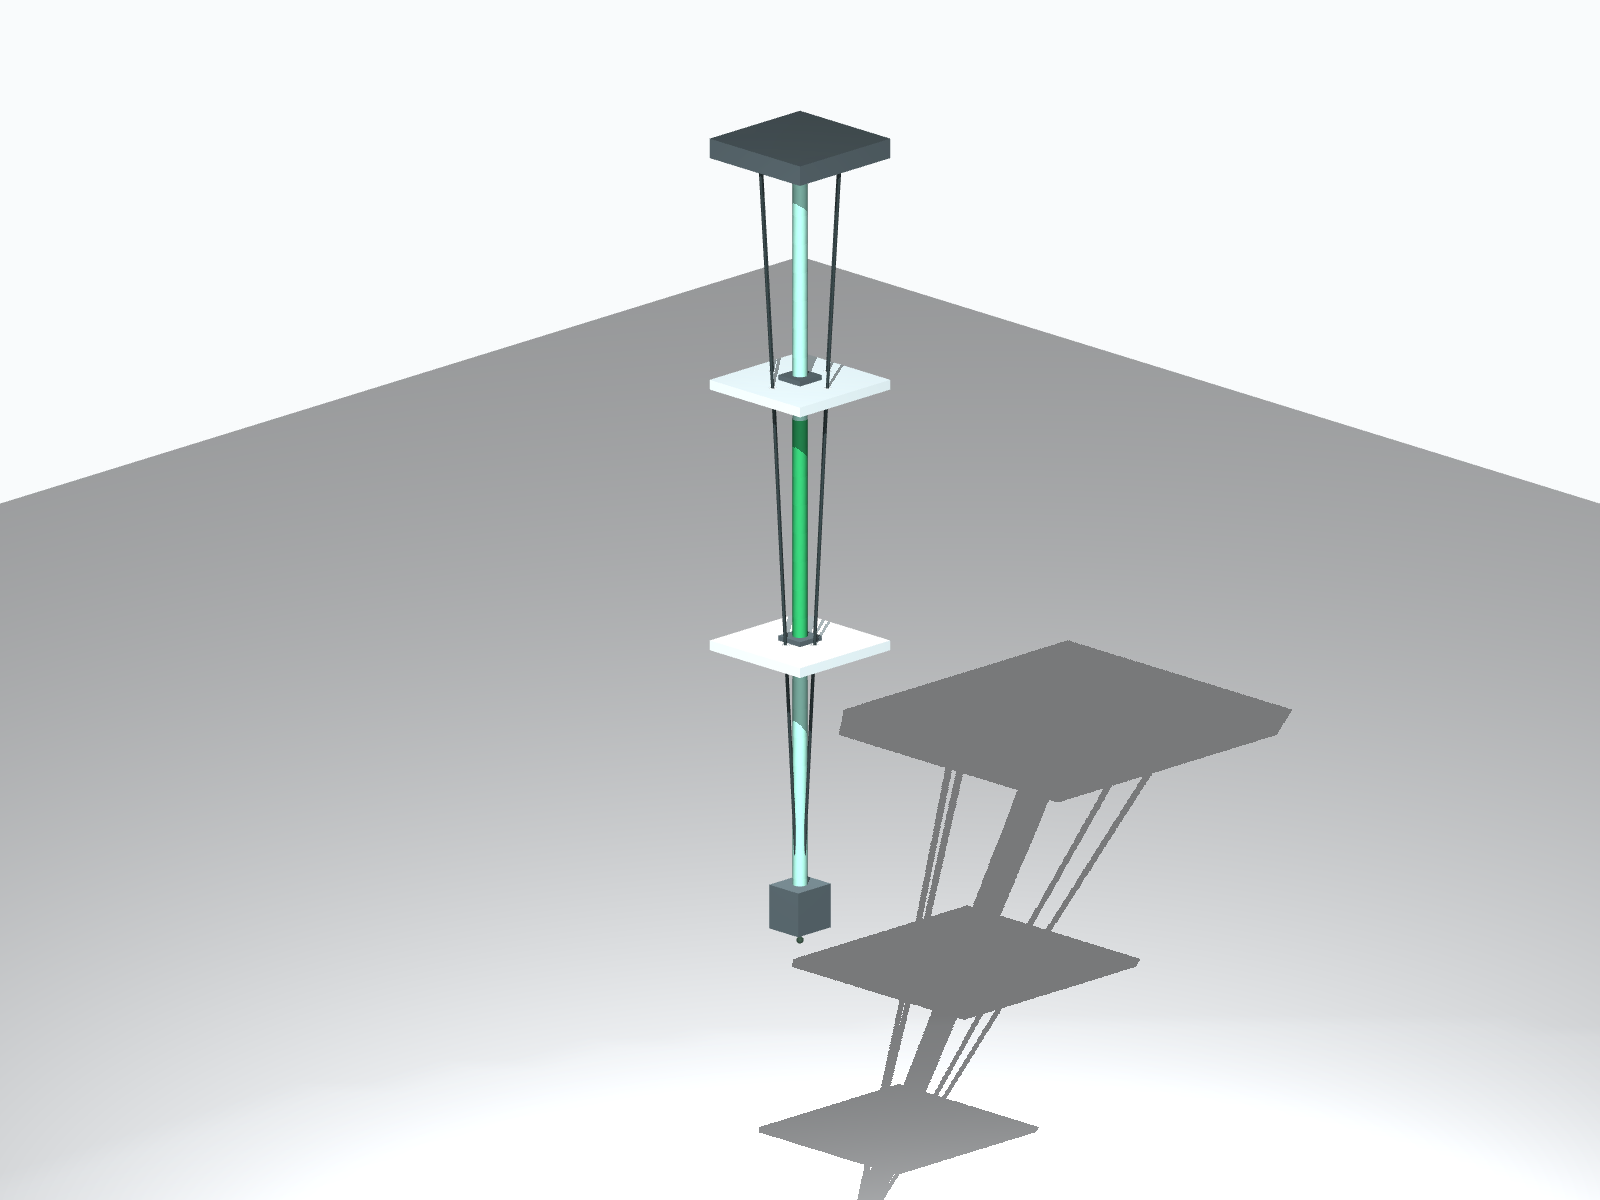
\includegraphics[width=\linewidth]{figures/native/phs2d_intermediate.png}
\par\footnotesize (b) Intermediate candidate
\par\scriptsize \textit{Action:} Revise tendon guidance
\end{minipage}\hfill
\begin{minipage}[t]{0.315\textwidth}\centering
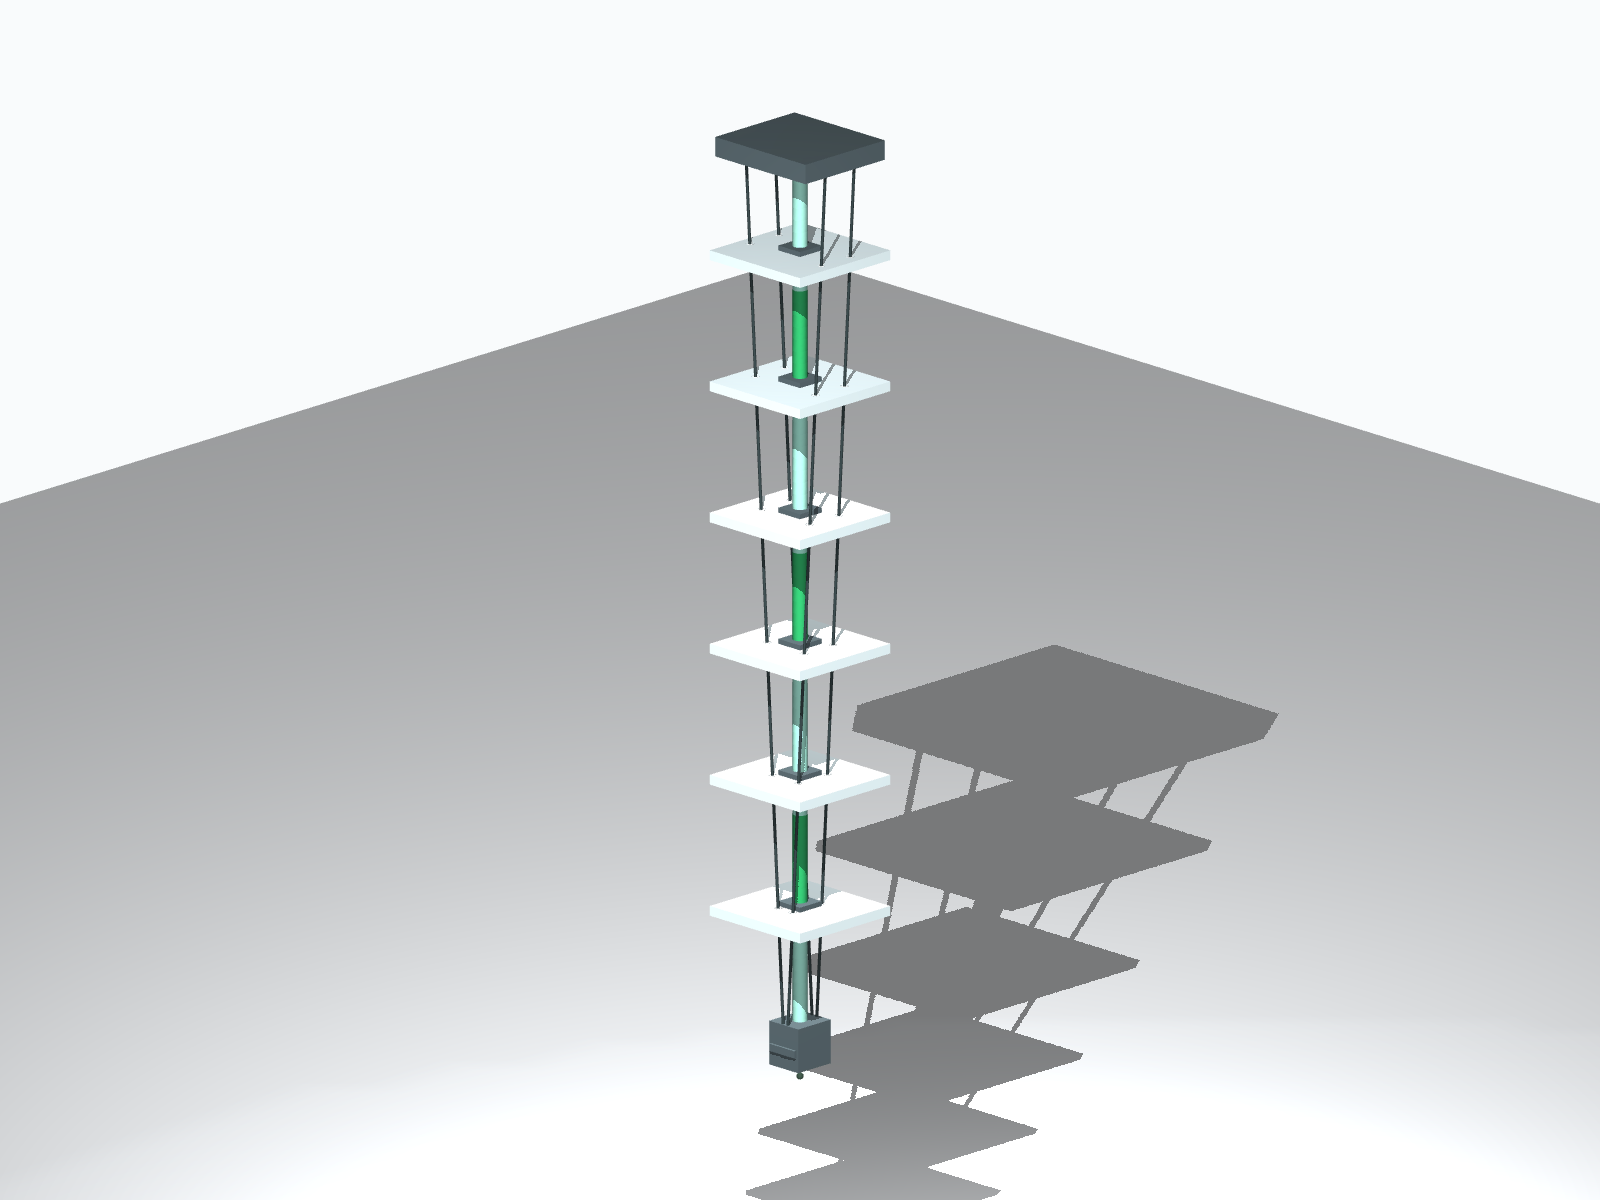
\includegraphics[width=\linewidth]{figures/native/phs2d_final.png}
\par\footnotesize (c) Accepted design
\par\scriptsize \textit{Physical test:} 10/10 loads pass
\end{minipage}
\par\vspace{5pt}
\begin{minipage}[t]{0.485\textwidth}\centering
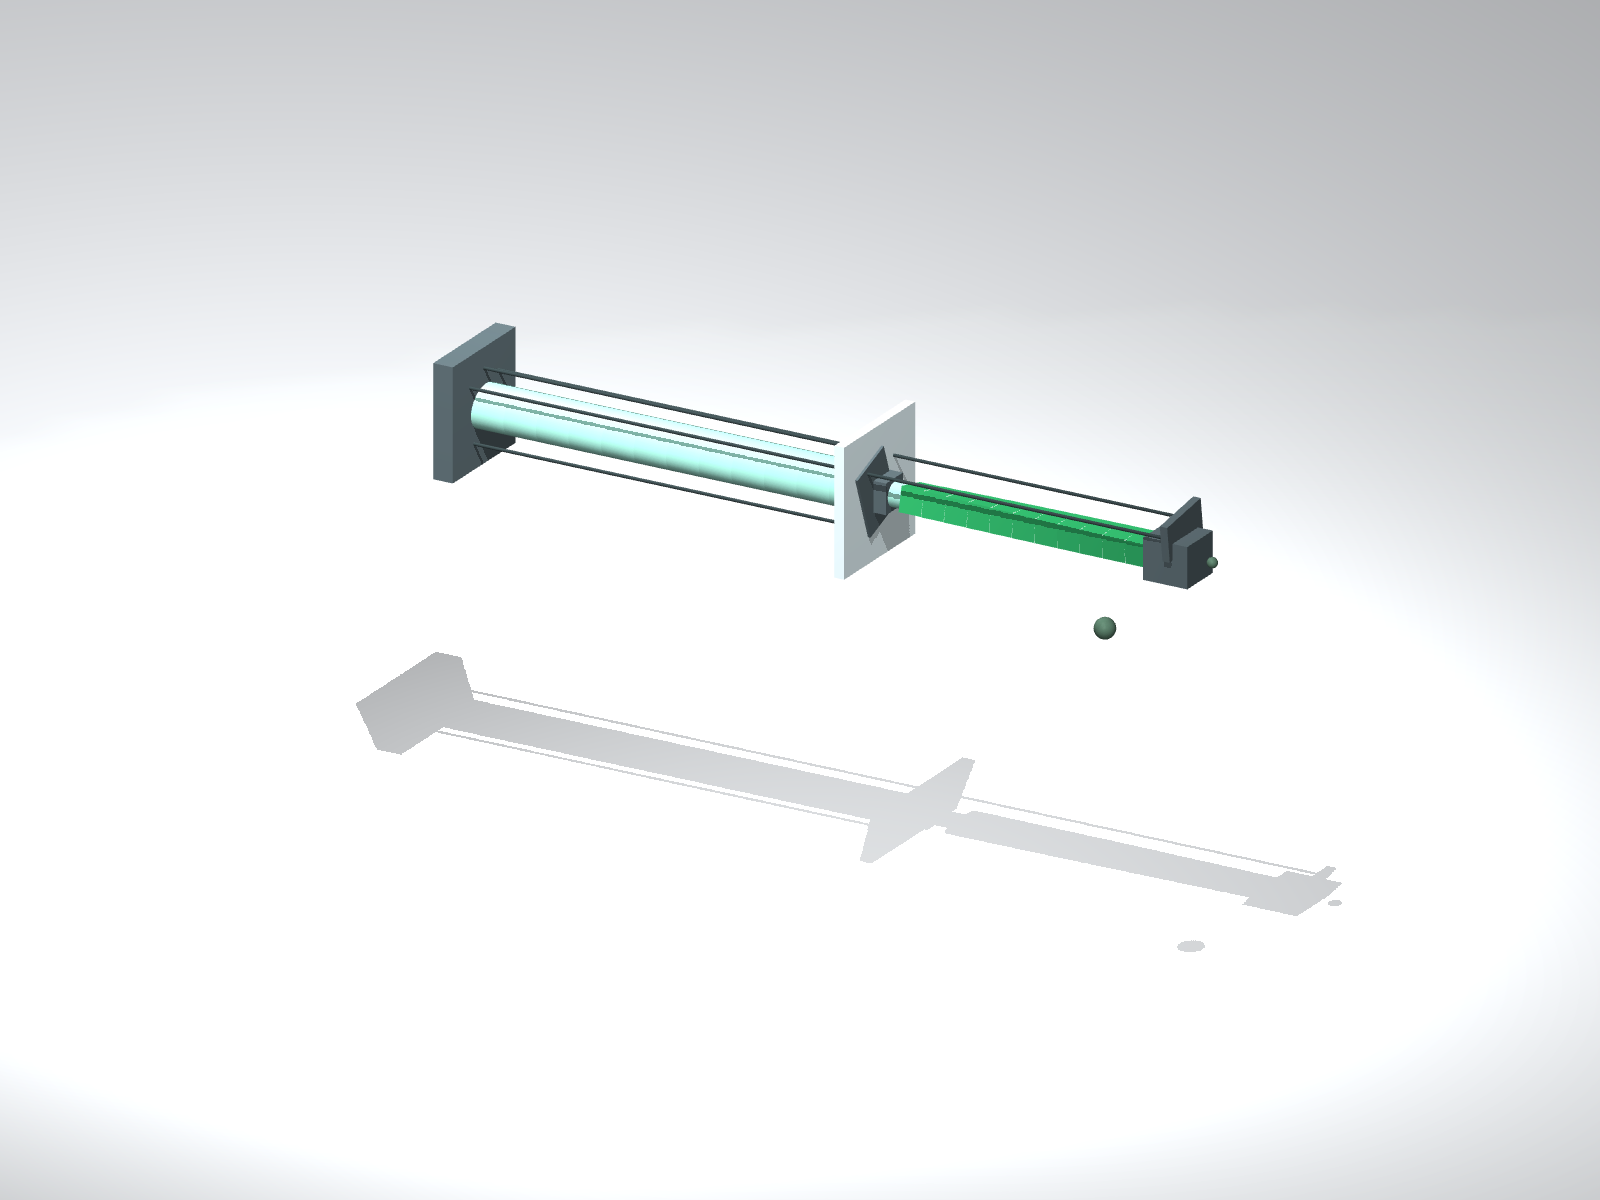
\includegraphics[width=\linewidth]{figures/native/t07_ellipse_root.png}
\par\footnotesize (d) Elliptical root candidate
\par\scriptsize \textit{Agent:} Test cross-plane coupling
\end{minipage}\hfill
\begin{minipage}[t]{0.485\textwidth}\centering
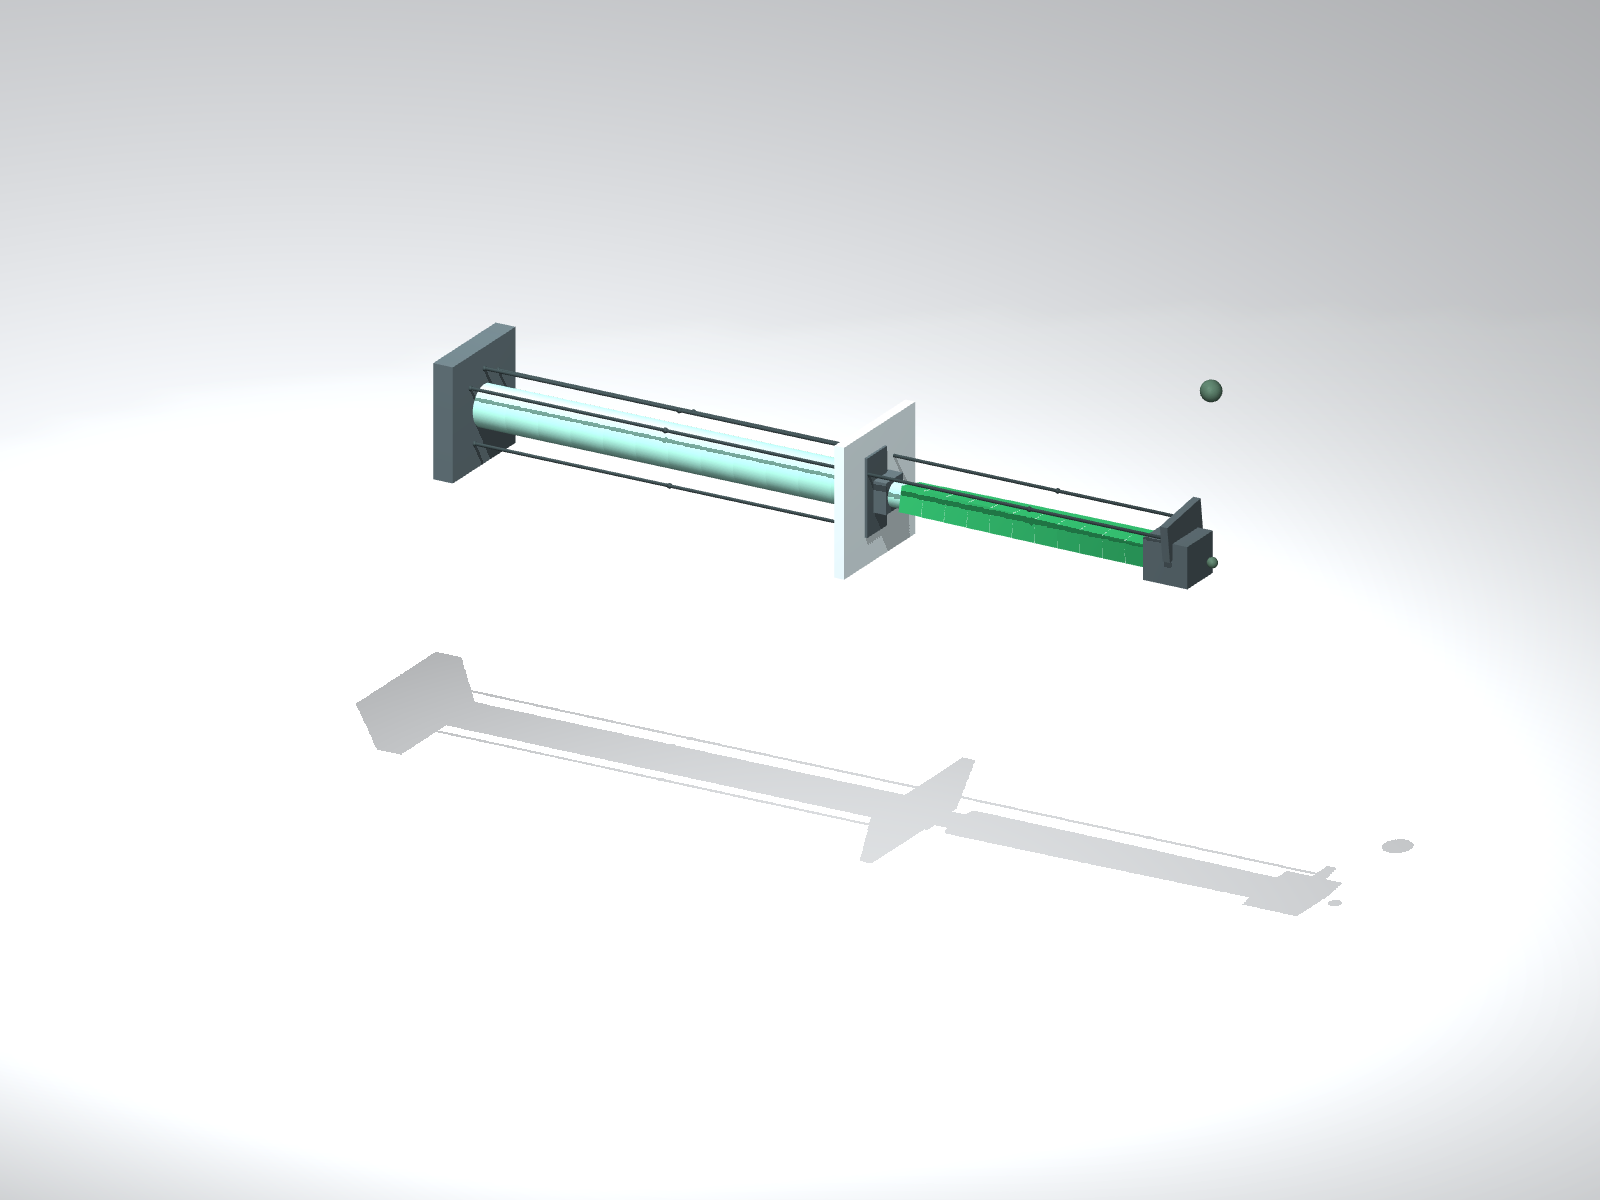
\includegraphics[width=\linewidth]{figures/native/t07_round_root.png}
\par\footnotesize (e) Final rounded-root morphology
\par\scriptsize \textit{Action:} Change root section and route
\par\scriptsize \textit{Physical test:} 4/4 conditions pass
\end{minipage}
\caption{Agent-guided structural evolution. Top: PHS-2D initial diagnostic, tendon-guidance revision, and accepted passive design. Bottom: T07 root-section hypothesis and revised common morphology. Each stage links a recorded structural action to physical evidence; images are native MuJoCo renders from archived models.}
\label{fig:structure-evolution}
\end{figure*}